\documentclass [xcolor=svgnames]{beamer} %svgnames import a bunch of colors
%to make black and white paste ", blackandwhite" inside brackets above (for transparencies)
\usetheme{Stockton}

%\usepackage{epsfig} %for figures
\usepackage{xcolor} %for color


\usepackage{listings}

\lstset{
  basicstyle=\small,
  basewidth=0.5em
}

\definecolor{hughesblue}{rgb}{.9,.9,1} %A blue I like to use for highlighting, matches Hughes Hallet's book



\title[ \hspace{4em}\insertframenumber/
\inserttotalframenumber]{~ {\large Bachelor Thesis:} \\ Interfacing TVLA and Sample\\~} %the [whatever] appears in the footer on the right


\author{ \\ Raphael Fuchs} %the [whatever] appears in the footer on the left

\date{April, 2011}

\begin{document}

\begin{frame}


\maketitle
\end{frame}

\begin{frame}
\frametitle{Outline}
\tableofcontents
\end{frame}

\section{Background}
\subsection{TVLA}
\begin{frame}
\frametitle{TVLA}
\textbf{T}hree-\textbf{V}alued-\textbf{L}ogic \textbf{A}nalyzer
\begin{columns}
  \begin{column}[l]{6cm}
\begin{itemize}
  \item ten years of track record in performing heap analyses
  \item proved to be quite powerful
  \item Heap structures and semantics of statements encoded with logical formulas (Kleene Logic)
  \item approximates heap safely as a bounded set of structures
  \item performs \textcolor{pacificblue}{summarization} and \textcolor{pacificblue}{materialization} of heap nodes, guided by user-specified \textcolor{pacificblue}{instrumentation predicates}
\end{itemize}
\end{column}
\begin{column}[r]{5cm}
\begin{center}
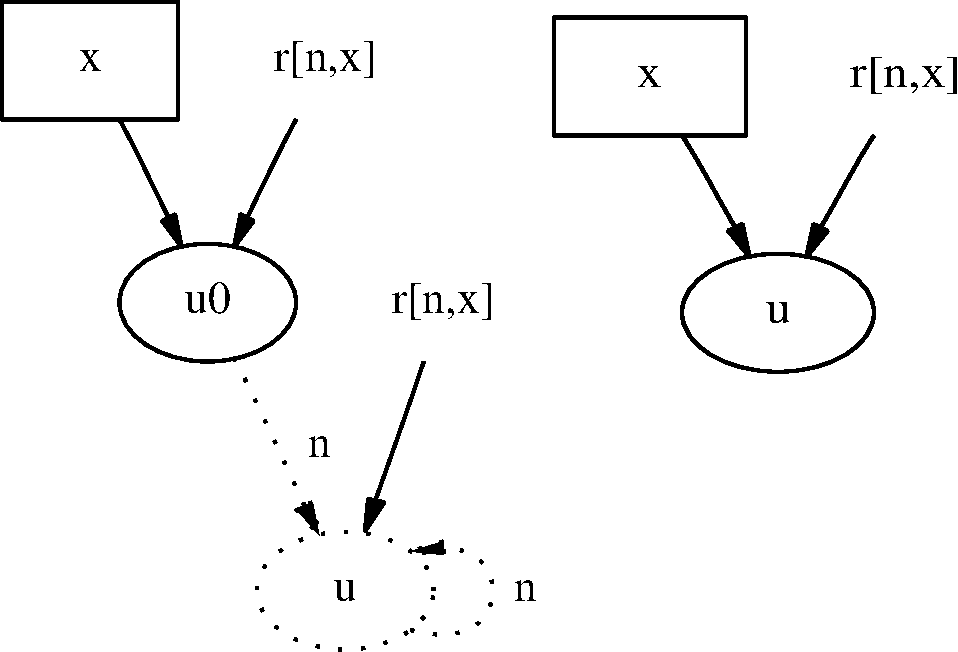
\includegraphics[width=5cm]{list.pdf}
\end{center}
\end{column}
\end{columns}
\end{frame}

\subsection{Sample} 
\begin{frame}
\frametitle{Sample}
\begin{itemize}
  \item Generic static analyzer
  \item Addresses multiple (object-oriented) languages
  \item Tracks different \textcolor{pacificblue}{abstract domains}
    \begin{itemize}
      \item Numerical information: Signs, intervals, octagons, polyhedra,\ldots
      \item Other Analyses: access permissions, type information,\ldots
      \item Heap domains: Heap identifiers pointed to by program variables.
    \end{itemize}
\end{itemize}
\pause
\bluebox{Current Heap Domains}{
\begin{blueitemize}
  \item Top domain: All references approximated by one heap identifier.
  \item Program-point bounded: For every program-point, keep at most one heap identifier.
\end{blueitemize}
}
\end{frame}

\section{Goal}
\begin{frame}
\frametitle{Goal}
\textbf{Sample needs a better heap domain!}

This involves coming up with
\begin{itemize}
  \item a representation of the heap (environment, heap identifiers)
  \item implementations of operations such as object creation, assignment, field access. 
\end{itemize}

\pause

Approach: For every statement that modifies the heap
\begin{itemize}
  \item encode the current heap as TVS (three-valued structures)
  \item let TVLA execute an action
  \item parse TVLA's output
  \item update representation in Sample

\end{itemize}
\end{frame}


\section{Challenges}
\begin{frame}[fragile]
\frametitle{Challenges}
\begin{itemize}
  \item<1-> TVLA model and Sample model are quite different.
    \begin{itemize}
      \item TVLA: unary/binary predicates
      \item Sample: we simply have heap identifiers and operations createObject, assign, fieldAccess etc.
    \end{itemize}
  \item<2-> Describe the semantics of Sample statements with TVLA \textcolor{pacificblue}{update formulae}
  \item<3-> Matching of input and output of TVLA: 
    \begin{itemize}
      \item We somehow have to give names to nodes
      \item Determine which heap nodes were summarized or materialized. 
    \end{itemize}
\item<4-> Optimize the way TVLA is invoked (efficiency)
  
\end{itemize}
\end{frame}


\section{Extensions}
\begin{frame}
\frametitle{Possible Extensions}

\grassgreenbox{
Supporting and Choosing Instrumentation Predicates
}{
\begin{itemize}
  \item \textcolor{pacificblue}{Instrumentation predicates} guide abstraction of the heap
  \item right choice is crucial to obtain precise results
  \item evaluation necessary
\end{itemize}
}
\pause
\grassgreenbox{
Benchmarking
}{
\begin{itemize}
  \item Apply analysis to a wide set of benchmarks
\end{itemize}
}
\pause
\grassgreenbox{
Predicates for Data Structures
}{
\begin{itemize}
  \item Develop specific predicates for data structures like lists and trees.
  \item May be useful to show that e.g ``list-ness'' is preserved by destructive updates.
\end{itemize}
}
\end{frame}

\begin{frame}
  \begin{center}
   \Huge{Questions?} 
  \end{center}
\end{frame}

\end{document}
